\chapter{Schur Polynomials}

Consider the following two representations of \(\sym_n\):
\begin{itemize}
    \item The trivial representation \(1 \colon \sym_n \to \GL_1(\complexes)\) given by \(\sigma \mapsto 1\).
    \item The sign representation \(\sign \colon \sym_n \to \GL_1(\complexes)\) given by \(\sigma \mapsto \sign(\sigma)\).
\end{itemize}

Consider any representation \(\phi \colon  \sym_n \to \GL_1(\complexes)\).
Let \(i \in \interval{n-1}\).
Then,
\begin{equation}
    \phi(\eltr{i}) = \phi(\tau \eltr{1} \tau^{-1}) = \phi(\tau) \phi(\eltr{1}) \phi(\tau)^{-1} = \phi(\eltr{1}),
\end{equation}
for some \(\tau \in \sym_n\).
Thus, \(\phi(\eltr{i})\) is independent of \(i\).
Moreover, \(\phi(\eltr{i})^2 = \phi(\eltr{i}^2) = \phi(\operatorname{id}) = 1\), hence \(\phi(\eltr{i}) = \pm 1\), for all \(i \in \interval{n-1}\).
If \(\phi(\eltr{i}) = 1\) for all \(i \in \interval{n-1}\), then \(\phi = 1\).
If \(\phi(\eltr{i}) = -1\) for all \(i \in \interval{n-1}\), then \(\phi = \sign\).

Therefore, the only irreducible representations of \(\sym_n\) of dimension \(1\) are the trivial representation and the sign representation.

Suppose \(\rho \colon \sym_n \to \GL(V)\) is a representation of \(S_n\).
The \vocab{invariants} of \(\rho\) are the elements \(v \in v\) such that
\begin{equation}
    \rho(w) v = 1(w) v, 
\end{equation}
for all \(w \in S_n\), where \(1\) denotes the trivial representation.
We can alternatively call these elements \vocab{\(1\)-isotypic elements}.
Let \(\Inv(V)\) denote the set of \(1\)-isotypic elements of \(\rho \colon S_n \to \GL(V)\).

We can replace the trivial representation with the sign representation.

The \vocab{\(\sign\)-isotypic elements} of \(\rho\) are the elements \(v \in V\) such that
\begin{equation}
    \rho(w) v = \sign(w) v,
\end{equation}
for all \(w \in S_n\).
Let \(\Alt(V)\) denote the set of \(\sign\)-isotypic elements of \(\rho \colon S_n \to \GL(V)\).

\begin{proposition}
    Let \(\rho \colon S_n \to \GL(V)\) be a representation of \(S_n\).
    Then, \(\Alt(V)\) is a subspace of \(V\).
\end{proposition}

\begin{definition}[Direct sum of representations]
    If \(\rho_1 \colon S_n \to \GL(V_1)\) and \(\rho_2 \colon S_n \to \GL(V_2)\) are representations of \(S_n\),
    then the \vocab{direct sum} of \(\rho_1\) and \(\rho_2\) is the representation \(\rho_1 \oplus \rho_2 \colon S_n \to \GL(V_1 \oplus V_2)\) given by
    \begin{equation}
        (\rho_1 \oplus \rho_2)(w) = \rho_1(w) \oplus \rho_2(w),
    \end{equation}
    for all \(w \in S_n\).
\end{definition}

Much more interesting than adding two representations to get a third,
is to start with a representation and decompose it into a direct sum of other representations.

\begin{theorem}
    Let \(\rho \colon S_n \to \GL(V)\) be a representation of \(S_n\).
    Then, \(V = \Inv(V) \oplus \Alt(V) \oplus W\), for some \(W \subset V\),
    and 
    \begin{equation}
        \rho = 1_{\Inv(V)} \oplus \sign_{\Alt(V)} \oplus \rho|_W.
    \end{equation}
\end{theorem}

We saw that, if \(V\) is an algebra, then \(\Inv(V)\) is a subalgebra of \(V\).
However, this is not the case for \(\Alt(V)\).
Suppose \(a \in \Alt(V)\).
Then \(w \cdot a^2 = (w \cdot a) (w \cdot a) = \sign(w)^2 a^2 = a^2\), for all \(w \in S_n\), which is not always equal to \(\sign(w) a^2\) (for \(n \geq 2\)).
Something can be salvaged from this situation.

\begin{theorem} \label{thm:inv-alt-subalgebra}
    Let \(V\) be an algebra.
    Let \(\rho \colon S_n \to \Aut(V)\) be a representation of \(S_n\).
    Consider the subspace \(\Inv(V) \oplus \Alt(V)\) of \(V\).
    Then, \(\Inv(V) \oplus \Alt(V)\) is a subalgebra of \(V\).
\end{theorem}

The proof of Theorem~\ref{thm:inv-alt-subalgebra} follows from Theorem~\ref{thm:inv-alt-super}.

\begin{definition}[\(G\)-graded algebra]
    A \vocab{\(G\)-graded algebra} is an algebra \(V\) together with a direct sum decomposition
    \begin{equation}
        V = \bigoplus_{g \in G} V_g,
    \end{equation}
    such that \(ab \in V_{gh}\), for all \(a \in V_g\) and \(b \in V_h\).
\end{definition}

A \vocab{superalgebra} is a \(\mathbb{Z}_2\)-graded algebra.

\begin{theorem} \label{thm:inv-alt-super}
    Let \(V\) be an algebra.
    Let \(\rho \colon S_n \to \Aut(V)\) be a representation of \(S_n\).
    Consider the subspace \(\Inv(V) \oplus \Alt(V)\) of \(V\).
    Then, \(\Inv(V) \oplus \Alt(V)\) is a superalgebra with parts \(\Inv(V)\) and \(\Alt(V)\).
\end{theorem}

\begin{proof}
    Let \(a \in \Inv(V)\) and \(b \in \Inv(V)\).
    Then, \(w \cdot (ab) = (w \cdot a) (w \cdot b) = a b\), for all \(w \in S_n\).
    Thus, \(ab \in \Inv(V)\).
    Let \(a \in \Inv(V)\) and \(b \in \Alt(V)\).
    Then, \(w \cdot (ab) = (w \cdot a) (w \cdot b) = (\sign(w) a) b = \sign(w) a b\), for all \(w \in S_n\).
    Thus, \(ab \in \Alt(V)\).
    Let \(a \in \Alt(V)\) and \(b \in \Alt(V)\).
    Then, \(w \cdot (ab) = (w \cdot a) (w \cdot b) = \sign(w)^2 a b = a b\), for all \(w \in S_n\).
    Thus, \(ab \in \Inv(V)\).

    Therefore, \(\Inv(V) \oplus \Alt(V)\) is a subalgebra of \(V\),
    and \(\Inv(V) \oplus \Alt(V)\) is a superalgebra with parts \(\Inv(V)\) and \(\Alt(V)\).
\end{proof}

Now, apply this with \(\mathcal{A} = \rationals[x_1, x_2, \ldots, x_n]\),
and the action \(\rho \colon S_n \to \Aut(\mathcal{A})\) given by
permuting the variables.
The \(\sign\)-isotypic elements of \(\mathcal{A}\) are are the \vocab{alternating polynomials},
denoted by \(\AltPoly(n)\) or \(v_n\Sym(n)\).

For example,
\begin{equation}
    x_1^2x_2 - x_2^2x_1 + x_2^2x_3 - x_3^2x_2 + x_3^2x_1 - x_1^2x_3 \in \AltPoly(3).
\end{equation}

\begin{lemma}
Let \(p \in \AltPoly(n)\).
Let \(\alpha\) be a composition of length \(n\).
Assume that \(\alpha_i = \alpha_j\) for some distinct \(i, j \in \interval{n}\).
Then, the coefficient of \(x^\alpha\) in \(p\) is zero.
\end{lemma}

\begin{proof}
    We compute that     
    \begin{equation}
        [x^\alpha] p = [x^alpha] (- \eltr{i, j} \cdot p) = - [x^\alpha] p,
    \end{equation}
    which implies that \([x^\alpha] p = 0\).
\end{proof}

\begin{definition}[Vandermonde polynomial]
    Define the \vocab{\(n\)\textsuperscript{th} Vandermonde polynomial} to be
    \begin{equation}
        v_n = \prod_{1 \leq i < j \leq n} (x_j - x_i) \in \AltPoly(n).
    \end{equation}
\end{definition}

\begin{lemma} \label{lem:vandermonde-divides-alt}
    Let \(p \in \AltPoly(n)\).
    Then, \(v_n \mid p\).
\end{lemma}

\begin{proof}
    Let \(i < j\) in \(\interval{n}\).
    If we specialize \(p\) by setting \(x_i = x_j\), then \(p \mapsto 0\).
    Therefore, \(x_i - x_j \mid p\).
    Since this holds for all \(i < j\), we have \(v_n \mid p\).
\end{proof}

\begin{lemma} \label{lem:vandermonde-times-sym-is-alt}
    Let \(p \in \AltPoly(n)\).
    Then, \(\frac{p}{v_n} \in \Sym(n)\).
\end{lemma}

\begin{proof}
    Let \(p \in \AltPoly(n)\).
    Then, \(p = v_n q\), for some \(q \in \rationals[x_1, x_2, \ldots, x_n]\),
    by Lemma~\ref{lem:vandermonde-divides-alt}.
    Since \(p, v_n \in \AltPoly(n)\),
    we have \(w \cdot p = \sign(w) p\) and \(w \cdot v_n = \sign(w) v_n\), for all \(w \in S_n\).
    Thus, \(w \cdot q = q\), for all \(w \in S_n\), and consequently, \(q \in \Sym(n)\).
\end{proof}

\begin{corollary}
    The map from \(\Sym(n)\) to \(\AltPoly(n)\) given by \(q \mapsto v_n q\) is a vector space isomorphism.
\end{corollary}

Note that bases of \(\Sym(n)\), multiplied by \(v_n\), form a basis of \(\AltPoly(n)\), and conversely, bases of \(\AltPoly(n)\), divided by \(v_n\), form a basis of \(\Sym(n)\).

Let's make one basis of \(\AltPoly(n)\) explicitly.

Given a partition \(\lambda\) of \(n\),
we define
\begin{equation}
    \tilde{a}_\lambda
    =
    \sum_{w \in \sym_n}
    \sign(w)
    x^{w \cdot \lambda} \in \AltPoly(n).
\end{equation}
Note that, if \(\lambda\) has equal parts, then \(\tilde{a}_\lambda = 0\).
A \vocab{strict partition} is a partition with distinct parts.
The set 
\begin{equation}
    \{ \tilde{a}_\lambda \mid \lambda \text{ is a strict partition of } n \}
\end{equation}
is a basis of \(\AltPoly(n)\).

Let \(\delta_n = (n-1, n-2, \ldots, 1, 0)\).
Note that the map \(\lambda \mapsto \lambda + \delta_n\) is a bijection between strict partitions of \(n\) and partitions of \(n+1\).
Then, we define
\begin{equation}
    a_\lambda = \tilde{a}_{\lambda + \delta_n} \in \AltPoly(n+1),
\end{equation}
and consequently, 
\begin{equation}
    \{ a_\lambda \mid \lambda \in \Par(n) \}
\end{equation}
is a basis of \(\AltPoly(n+1)\).

If we have a basis of \(\AltPoly(n)\),
we can divide by \(v_n\) to get a basis of \(\Sym(n)\).

\begin{definition}[Schur polynomial]
    Let \(\lambda\) be a partition of \(n\).
    Define the \vocab{Schur polynomial} \(s_\lambda \in \Sym(n)\) by
    \begin{equation}
        s_\lambda = \frac{a_\lambda}{v_n} \in \Sym(n).
    \end{equation}
\end{definition}

\begin{proposition}[Jacobi's bialternant formula]
    Let \(\lambda\) be a partition of \(n\).
    Then,
    \begin{equation}
        s_\lambda = 
        \frac{
            \det\left(\left[x_i^{\lambda_j + n - j}\right]\right)_{i, j \in \interval{n}}
        }{
            \det\left(\left[x_i^{n - j}\right]\right)_{i, j \in \interval{n}}
        }.
    \end{equation}
\end{proposition}

\begin{example}[\(n = 3\), \(\lambda  = \composition{2}\)]
    Let \(n = 3\).
    Then, \(\delta_3 = \composition{2, 1, 0}\)
    and
    \begin{equation}
        v_3 = a_{\composition{0, 0, 0}} = \tilde{a}_{\composition{2, 1, 0}} = x_1^2x_2 - x_2^2x_1 + x_2^2x_3 - x_3^2x_2 + x_3^2x_1 - x_1^2x_3.
    \end{equation}
    Moreover, for \(\lambda = \composition{2}\),
    we have
    \begin{align}
        s_{\composition{2}}
        = \frac{a_{\composition{2}}}{v_3}
        = \frac{\tilde{a}_{\composition{4, 1, 0}}}{\tilde{a}_{\composition{2, 1, 0}}}
        &= \frac{
            x_{1}^{4} x_{2} - x_{2}^{4} x_{1} +
            x_{2}^{4} x_{3} - x_{3}^{4} x_{2} +
            x_{3}^{4} x_{1} - x_{1}^{4} x_{3}
        }{
            x_{1}^{4} x_{2} - x_{2}^{4} x_{1} +
            x_{2}^{4} x_{3} - x_{3}^{4} x_{2} +
            x_{3}^{4} x_{1} - x_{1}^{4} x_{3}
        } \\
        &= x_1^2 + x_2^2 + x_3^2 + x_1x_2 + x_2x_3 + x_3x_1 = h_2.
    \end{align}
\end{example}

\begin{example}[\(n = 3\), \(\lambda  = \composition{1, 1}\)]
    Let \(n = 3\) and \(\lambda = \composition{1, 1}\).
    :We have
    \begin{align}
        s_{\composition{1, 1}}
        = \frac{a_{\composition{1, 1}}}{v_3}
        = \frac{\tilde{a}_{\composition{3, 2, 0}}}{\tilde{a}_{\composition{2, 1, 0}}}
        &= \frac{
            x_{1}^{3} x_{2}^{2} - x_{2}^{3} x_{1}^{2} +
            x_{2}^{3} x_{3}^{2} - x_{3}^{3} x_{2}^{2} +
            x_{3}^{3} x_{1}^{2} - x_{1}^{3} x_{3}
        }{
            x_{1}^{3} x_{2}^{2} - x_{2}^{3} x_{1}^{2} +
            x_{2}^{3} x_{3}^{2} - x_{3}^{3} x_{2}^{2} +
            x_{3}^{3} x_{1}^{2} - x_{1}^{3} x_{3}^{2}
        } \\
        &= x_1x_2 + x_2x_3 + x_3x_1 = e_2.
    \end{align}
\end{example}

Although it is a pain to write out Schur polynomials explicitly,
we know that
\begin{itemize}
    \item \(s_\lambda\) has integer coefficients, by divisibility rules on monic polynomials,
    \item \(s_\lambda\) is an integral linear combination of \(m_\mu\)'s, and \(m_\mu\)'s are integral linear combinations of \(s_\lambda\)'s.
\end{itemize}

\section{Pieri's Formulas and Strips}

\begin{definition}[Horizontal and vertical strips]
    A \vocab{horizontal strip} is a set of boxes in a Young diagram
    such that at most one box is in each column.
    A \vocab{vertical strip} is a set of boxes in a Young diagram
    such that at most one box is in each row.
\end{definition}

For example, the empty set is both a horizontal and vertical strip.

\begin{theorem}[Pieri's \(e\)-formula] \label{thm:pieri-e-formula}
    Let \(\lambda\) be a partition.
    Then,
    \begin{equation}
        s_\lambda e_k = \sum_{\mu} s_{\mu},
    \end{equation}
    where the sum is over all partitions \(\mu\) obtained by adding a vertical strip of size \(k\) to \(\lambda\).
\end{theorem}

\begin{proof}
    Note that
    \begin{align}
        \tilde{a}_{\lambda + \delta_n} e_k
        &=
        \left(
            \sum_{w \in \sym_n} \sign(w) x^{w \cdot (\lambda + \delta_n)} 
        \right) 
        \left(
            \sum_{i_1 < i_2 < \cdots < i_k} x_{i_1} x_{i_2} \cdots x_{i_k}
        \right) \\
        &=
        \sum_{w \in \sym_n}
        \sum_{\substack{\text{binary compositions } \alpha \\ \text{of } k \text{ with length } n}}
        \sign(w) x^{w \cdot (\lambda + \delta_n) + \alpha} \\
        &=
        \sum_{w \in \sym_n}
        \sum_{\substack{\text{binary compositions } \alpha \\ \text{of } k \text{ with length } n}}
        \sign(w) x^{w \cdot (\lambda + \delta_n + \alpha)} \\
        &=
        \sum_{\substack{\text{binary compositions } \alpha \\ \text{of } k \text{ with length } n}}
        \sum_{w \in \sym_n}
        \sign(w) x^{w \cdot (\lambda + \delta_n + \alpha)} \\
        &=
        \sum_{\substack{\text{binary compositions } \alpha \\ \text{of } k \text{ with length } n}}
        \tilde{a}_{\lambda + \alpha + \delta_n}.
    \end{align}

    Recall that, \(\tilde{a}_{\lambda + \alpha + \delta_n} = 0\) if \(\lambda + \alpha + \delta_n\) has equal parts.
    Using that \(\alpha\) has entries \(0\) or \(1\), this happens whenever \(\lambda + \alpha\) is not a partition.
    Therefore, add the condition the sum that \(\lambda + \alpha\) is a partition, that is,
    \begin{align}
        \tilde{a}_{\lambda + \delta_n} e_k
        &= \sum_{\substack{\text{binary compositions } \alpha \\ \text{of } k \text{ with length } n \\ \lambda + \alpha \text{ is a partition}}}
        \tilde{a}_{\lambda + \alpha + \delta_n} \\
        &= \sum_{\substack{\text{partitions } \mu \\ \lambda - \mu \text{ is a binary composition of } k}}
        \tilde{a}_{\mu + \delta_n}.
    \end{align}

    Therefore,
    \begin{equation}
        a_\lambda e_k = \sum_{\mu} a_{\mu},
    \end{equation}
    where the sum is over all partitions \(\mu\) obtained by adding a vertical strip of size \(k\) to \(\lambda\).
    Finally, the result follows by dividing by \(v_n\).
\end{proof}

\begin{corollary}
    Let \(k\) be a nonnegative integer.
    Then,
    \begin{equation}
        s_{\composition{1}^k} = e_k.
    \end{equation}
\end{corollary}

Note that this is somewhat similar to the formula
\begin{equation}
    e_{\lambda} e_k = e_{\operatorname{sort}(\lambda, k)}.
\end{equation}

\begin{theorem}[Pieri's \(h\)-formula] \label{thm:pieri-h-formula}
    Let \(\lambda\) be a partition.
    Then,
    \begin{equation}
        s_\lambda h_k = \sum_{\mu} s_{\mu},
    \end{equation}
    where the sum is over all partitions \(\mu\) obtained by adding a horizontal strip of size \(k\) to \(\lambda\).
\end{theorem}

\begin{proof}
    Note that
    \begin{align}
        \tilde{a}_{\lambda + \delta_n} h_k
        &=
        \left(
            \sum_{w \in \sym_n} \sign(w) x^{w \cdot (\lambda + \delta_n)} 
        \right) 
        \left(
            \sum_{i_1 \leq i_2 \leq \cdots \leq i_k} x_{i_1} x_{i_2} \cdots x_{i_k}
        \right) \\
        &=
        \sum_{w \in \sym_n}
        \sum_{\substack{\text{compositions } \alpha \\ \text{of } k \text{ with length } n}}
        \sign(w) x^{w \cdot (\lambda + \delta_n) + \alpha} \\
        &=
        \sum_{w \in \sym_n}
        \sum_{\substack{\text{compositions } \alpha \\ \text{of } k \text{ with length } n}}
        \sign(w) x^{w \cdot (\lambda + \delta_n + \alpha)} \\
        &=
        \sum_{\substack{\text{compositions } \alpha \\ \text{of } k \text{ with length } n}}
        \sum_{w \in \sym_n}
        \sign(w) x^{w \cdot (\lambda + \delta_n + \alpha)} \\
        &=
        \sum_{\substack{\text{compositions } \alpha \\ \text{of } k \text{ with length } n}}
        \tilde{a}_{\lambda + \delta_n + \alpha}.
    \end{align}

    We define an involution on the set \(\mathcal{B}\) of compositions \(\alpha\) of \(k\) with length \(n\) such that the boxes of the Young diagram of \(\lambda + \alpha\) that are not in the Young diagram of \(\lambda\) do not form a horizontal strip.
    (The notation \(\mathcal{B}\) stands for \emph{bad}.)

    Let \(\alpha \in \mathcal{B}\).
    Since the boxes of the Young diagram of \(\lambda + \alpha\) that are not in the Young diagram of \(\lambda\) do not form a horizontal strip,
    there exists \(i\) such that
    \(\alpha_{i+1} > \lambda_i - \lambda_{i+1}\).
    Then, \(\lambda + \alpha\) is not a partition.
    Choose the smallest such \(i\).
    Define \(\beta\) by
    \begin{gather}
        \beta_i = \alpha_{i+1} - (\lambda_i - \lambda_{i+1} + 1), \quad
        \beta_{i+1} = \alpha_i + (\lambda_i - \lambda_{i+1} + 1), \\
        \beta_j = \alpha_j \text{ for } j \notin \{i, i+1\}.
    \end{gather}

    For example, when \(\lambda = \composition{6, 4, 2, 2, 1}\) and \(\alpha = \composition{1, 2, 7, 2, 5}\),
    we have
    \(i = 2\) and \(\beta = \composition{1, 4, 5, 2, 5}\), as shown in Figure~\ref{fig:pieri-h-formula-involution}.

    \begin{figure}[htbp]
        \centering
        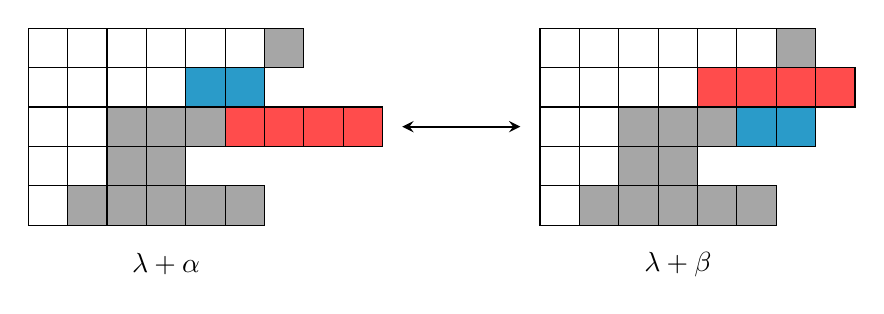
\begin{tikzpicture}[
                x=0.5cm, y=0.5cm,
                square/.style={draw, minimum size=0.5cm},
                white/.style={fill=white},
                gray/.style={fill=gray!70},
                blue/.style={fill=cyan!80!black},
                green/.style={fill=green!80!black},
                red/.style={fill=red!70!white}
            ]
            \begin{scope}[shift={(0,0)}]
                % First Row
                \foreach \x in {0,1,2,3,4,5} { \node[square, white] at (\x,4) {}; }
                \node[square, gray] at (6,4) {};
    
                % Second Row
                \foreach \x in {0,1,2,3} { \node[square, white] at (\x,3) {}; }
                \foreach \x in {4,5} { \node[square, blue] at (\x,3) {}; }
    
                % Third Row
                \foreach \x in {0,1} { \node[square, white] at (\x,2) {}; }
                \foreach \x in {2,3,4} { \node[square, gray] at (\x,2) {}; }
                \foreach \x in {5,6,7,8} { \node[square, red] at (\x,2) {}; }
    
                % Fourth Row
                \foreach \x in {0,1} { \node[square, white] at (\x,1) {}; }
                \foreach \x in {2,3} { \node[square, gray] at (\x,1) {}; }
    
                % Fifth Row
                \node[square, white] at (0,0) {};
                \foreach \x in {1,2,3,4,5} { \node[square, gray] at (\x,0) {}; }
            \end{scope}
            \node at (3, -1.5) {$\lambda + \alpha$};
            \begin{scope}[shift={(13,0)}] % Position of the second grid
                % First Row
                \foreach \x in {0,1,2,3,4,5} { \node[square, white] at (\x,4) {}; }
                \node[square, gray] at (6,4) {};
    
                % Second Row
                \foreach \x in {0,1,2,3} { \node[square, white] at (\x,3) {}; }
                \foreach \x in {4,5,6,7} { \node[square, red] at (\x,3) {}; }
    
                % Third Row
                \foreach \x in {0,1} { \node[square, white] at (\x,2) {}; }
                \foreach \x in {2,3,4} { \node[square, gray] at (\x,2) {}; }
                \foreach \x in {5,6} { \node[square, blue] at (\x,2) {}; }
    
                % Fourth Row
                \foreach \x in {0,1} { \node[square, white] at (\x,1) {}; }
                \foreach \x in {2,3} { \node[square, gray] at (\x,1) {}; }
    
                % Fifth Row
                \node[square, white] at (0,0) {};
                \foreach \x in {1,2,3,4,5} { \node[square, gray] at (\x,0) {}; }
            \end{scope}
            \node at (16, -1.5) {$\lambda + \beta$};
            \draw[<->, thick, >=stealth] (9,2) -- (12,2) node[midway, above] {};
    
        \end{tikzpicture}
        \caption{Example of the involution in the proof of Pieri's \(h\)-formula.}
        \label{fig:pieri-h-formula-involution}
    \end{figure}
    
    This map from \(\mathcal{B}\) to itself is an involution,
    and it satisfies that
        \(\lambda + \alpha + \delta_n\)
        \(\lambda + \beta + \delta_n\)
    differ by one transposition,
    hence
    \begin{equation}
        \tilde{a}_{\lambda + \alpha + \delta_n} + \tilde{a}_{\lambda + \beta + \delta_n} = 0.
    \end{equation}
    Finally,
    this implies that
    \begin{equation}
        \sum_{\alpha \in \mathcal{B}}
        \tilde{a}_{\lambda + \alpha + \delta_n}
        = 0,
    \end{equation}
    and consequently
    \begin{align}
        \tilde{a}_{\lambda + \delta_n} h_k
        &= \sum_{\substack{\text{compositions } \alpha \\ \text{of } k \text{ with length } n \\ (\lambda + \alpha) \setminus \lambda \text{ is a horizontal strip}}}
        \tilde{a}_{\lambda + \alpha + \delta_n} \\
        &= \sum_{\substack{\text{partitions } \mu \\ \lambda \setminus \mu \text{ is a Horizontal strip of size } k}}
        \tilde{a}_{\mu + \delta_n}.
    \end{align}
    Therefore,
    \begin{equation}
        a_\lambda h_k = \sum_{\mu} a_{\mu},
    \end{equation}
    where the sum is over all partitions \(\mu\) obtained by adding a horizontal strip of size \(k\) to \(\lambda\).
    Finally, the result follows by dividing by \(v_n\).
\end{proof}

In the next section, we solve a problem that we didn't even know we wanted to solve:
\emph{How to write \(h_\lambda\) and \(e_\lambda\) in the Schur basis?}

\section{Tableaux and Kostka Numbers}

\begin{definition}[Semistandard Young tableaux]
    A \vocab{semistandard tableaux \(T\)} 
    is a sequence of nested partitions
    \begin{equation}
        \varnothing = \lambda^{(0)}
        \subset \lambda^{(1)}
        \subset \cdots
        \subset \lambda^{(\ell)},
    \end{equation}
    such that \(\lambda^{(k)} \setminus \lambda^{(k-1)}\) is a horizontal strip, for all \(k \in \interval{\ell}\).
    We say that \(T\) has \vocab{shape} \(\lambda = \lambda^{(\ell)}\).
\end{definition}

Traditionally, a semistandard tableau \(T\) of shape \(\lambda\) is represented by filling the boxes of the diagram of \(\lambda\) with numbers from the set \(\{1, 2, \ldots, \ell\}\). Specifically, the number \(i\) is placed in the boxes corresponding to the horizontal strip \(\lambda^{(i)} \setminus \lambda^{(i-1)}\).

Under this depiction, a filling of the boxes of a Young diagram is semistandard if and only if the entries in each row are weakly increasing from left to right, and the entries in each column are strictly increasing from top to bottom.

\begin{example}
    Consider the following semistandard tableaux of shape \(\composition{5, 4, 2}\):
    \begin{equation}
        \varnothing
        \subset \composition{3}
        \subset \composition{4, 2}
        \subset \composition{4, 2}
        \subset \composition{5, 4}
        \subset \composition{5, 4, 2}.
    \end{equation}
    This tableaux is drawn as
    \begin{equation}
        \begin{ytableau}
            1 & 1 & 1 & 2 & 4 \\
            2 & 2 & 4 & 4 \\
            5 & 5
        \end{ytableau}.
    \end{equation}
\end{example}

The \vocab{weight} (sometimes called \vocab{content}) of a tableaux
is the composition \(\alpha\) such that the number \(i\) appears \(\alpha_i\) times in the tableaux, that is, \(\alpha_i\) is the size of the horizontal strip \(\lambda^{(i)} \setminus \lambda^{(i-1)}\).

\begin{definition}[Standard Young tableaux]
    A \vocab{standard tableaux} is a semistandard Young tableaux with weight \(\composition{1, 1, \ldots, 1}\), that is, each horizontal strip has size \(1\).
\end{definition}

\begin{definition}[Kostka numbers]
    Let \(\lambda\) be a partition and \(\alpha\) be a composition.
    The \vocab{Kostka number} \(K_{\lambda \alpha}\) is the number of standard Young tableaux of shape \(\lambda\) and weight \(\alpha\).
\end{definition}

\begin{theorem} \label{thm:h-e-sum-kostka-schur}
    Let \(\alpha\) be a composition.
    Then,
    \begin{equation}
        h_\alpha = \sum_{\lambda} K_{\lambda \alpha} s_\lambda,
    \end{equation}
    and
    \begin{equation}
        e_\alpha = \sum_{\lambda} K_{\lambda \alpha} s_{\tilde\lambda}.
    \end{equation}
\end{theorem}

\begin{proof}
    Note that 
    \begin{align}
        h_\alpha
        &= h_{\alpha_1} h_{\alpha_2} \cdots h_{\alpha_\ell} \\
        &= s_{\varnothing} h_{\alpha_1} s_{\varnothing} h_{\alpha_2} \cdots s_{\varnothing} h_{\alpha_\ell},
    \end{align}
    and then the result follows by successively applying \nameref{thm:pieri-h-formula}.
    The proof for the \(e\)-formula is similar, using \nameref{thm:pieri-e-formula}.
\end{proof}

We list some observations about Kostka numbers.

\begin{corollary} \label{cor:kostka-composition-sort}
    Let \(\alpha\) be a composition and let \(\mu = \overline{\alpha}\).
    Then, \(K_{\lambda \alpha} = K_{\lambda \mu}\).
\end{corollary}

\begin{proof}
    Since \(h_\alpha = h_\mu\), the result follows from Theorem~\ref{thm:h-e-sum-kostka-schur} and the fact that the Schur polynomials are linearly independent.
\end{proof}

\begin{fact}
    If \(|\lambda| \neq |\mu|\), then \(K_{\lambda \mu} = 0\).
\end{fact}

\begin{fact}
    Let \(\lambda\) be a partition.
    Then \(K_{\lambda \lambda} = 1\).
\end{fact}

The only standard Young tableaux of shape \(\lambda\) and weight \(\lambda\) is the one where the number \(i\) is placed in the \(i\)\textsuperscript{th} box of the \(i\)\textsuperscript{th} row.
This tableaux is called \vocab{Yamanouchi tableaux}, \vocab{the highest weight tableaux of shape \(\lambda\)}, or \vocab{supersemistandard tableaux}.

\begin{fact}
    Let \(\lambda, \mu\) be partitions.
    If \(K_{\lambda \mu} \neq 0\), then \(\lambda \geq \mu\).
\end{fact}

\begin{proof}
    Let \(i\) be a positive integer.
    The entries of a standard Young tableaux of shape \(\lambda\) and weight \(\mu\) that are at most \(i\) must be contained in the first \(i\) rows of the Young diagram of \(\lambda\).
    Therefore, \(\lambda_1 + \cdots + \lambda_i \geq \mu_1 + \cdots + \mu_i\) for all \(i\),
    and consequently, \(\lambda \geq \mu\).
\end{proof}

\begin{fact}
    Kostka numbers are not symmetric, that is, 
    there exist partitions \(\lambda, \mu\) such that \(K_{\lambda \mu} \neq K_{\mu \lambda}\).
\end{fact}

\begin{example}
    Let \(\lambda = \composition{2}\) and \(\mu = \composition{1, 1}\).
    Then, \(K_{\lambda \mu} = 1\) and \(K_{\mu \lambda} = 0\).
\end{example}

The \vocab{Kostka matrix} \(K\) is the matrix where the entry in the \(\mu\)\textsuperscript{th} row and \(\lambda\)\textsuperscript{th} column is \(K_{\lambda \mu}\) (note the reversal of indices).
Note that \(K\) is upper triangular (with respect a linear extension of the dominance order) and its diagonal entries are all \(1\).
Therefore, \(K\) is invertible, and its inverse has integer entries.
We call \(K^{-1}\) the \vocab{inverse Kostka matrix}.
Let \(K^{-1}_{\lambda \mu}\) be the entry in the \(\mu\)\textsuperscript{th} row and \(\lambda\)\textsuperscript{th} column of \(K^{-1}\).

\begin{theorem}
    Let \(\lambda\) be a partition.
    Then,
    \begin{equation}
        \omega(s_\lambda) = s_{\tilde\lambda}.
    \end{equation}
\end{theorem}

\begin{proof}
    Theorem~\ref{thm:h-e-sum-kostka-schur} implies that
    \begin{equation}
        s_\lambda = \sum_{\mu} K_{\lambda \mu}^{-1} h_\mu,
    \end{equation}
    and 
    \begin{equation}
        s_{\tilde\lambda} = \sum_{\mu} K_{\lambda \mu}^{-1} e_\mu.
    \end{equation}
    It is straightforward to check that applying \(\omega\) to the right-hand side of the first equation gives the right-hand side of the second equation, and the result follows.
\end{proof}

\begin{theorem}[Jacobi--Trudi's determinant formula] \label{thm:jacobi-trudi}
    Let \(\lambda\) be a partition and let \(n \geq \ell(\lambda)\) be an integer.
    Then,
    \begin{equation}
        s_\lambda = \det\left( s_{\lambda_i + n - i - j} \right)_{i, j \in \interval{n}}.
    \end{equation}
    and
    \begin{equation}
        s_{\tilde\lambda} = \det\left( s_{\lambda_i + n - i - j} \right)_{i, j \in \interval{n}}.
    \end{equation}
\end{theorem}

\begin{example}
    Let's compute \(s_{\composition{3, 1}}\) using \nameref{thm:jacobi-trudi}.
    Let \(n = 4\).
    We have
    \begin{equation}
        s_{\composition{3, 1}}
        = \left|
            \begin{matrix}
                h_3 & h_4 & h_5 & h_6 \\
                h_0 & h_1 & h_2 & h_3 \\
                0   & 0   & h_0 & h_1 \\
                0   & 0   & 0   & h_0
            \end{matrix}
        \right|
        = \left|
            \begin{matrix}
                h_3 & h_4 \\
                h_0 & h_1 \\
            \end{matrix}
        \right|
        = h_{\composition{3, 1}} - h_{\composition{4}},
    \end{equation}
    and
    \begin{equation}
        s_{\composition{3, 1}} = s_{\tilde{\composition{2, 1, 1}}} =
        \left|
            \begin{matrix}
                e_2 & e_3 & e_4 \\
                e_0 & e_1 & e_2 \\
                0   & e_0 & e_1
            \end{matrix}
        \right|
        = e_{\composition{2, 1, 1}} + e_{\composition{4}} - e_{\composition{3, 1}} - e_{\composition{2, 2}}.
    \end{equation}
\end{example}

\begin{proof}[Proof of \nameref{thm:jacobi-trudi}]
    It is straightforward to check that the determinants are equal for all \(n \geq \ell(\lambda)\). Therefore, it suffices to prove the result for \(n = \ell(\lambda)\).

    We proceed by induciton on \(n = \ell(\lambda)\).
    The result is true for \(n = 0\).

    We column expand along the rightmost column
    \begin{equation}
        \det\left( s_{\lambda_i + \ell - i - j} \right)_{i, j \in \interval{n}}
        =
        \sum_{i=1}^\ell
        (-1)^{\ell - i}
        h_{\lambda_i + \ell - i}
        s_{\composition{\lambda_1, \ldots, \lambda_{i-1}, \lambda_{i+1} - 1, \ldots, \lambda_\ell - 1}}
    \end{equation}

    \textcolor{red}{... I did not finish this proof. Reading a book proof might be better.}
\end{proof}

\begin{theorem}
    \begin{equation}
        \prod_{i, j} (1 - x_i y_j)^{-1} = \sum_{\lambda} s_\lambda(x) s_{\lambda}(y).
    \end{equation}
\end{theorem}

\begin{proof}
    By \nameref{thm:jacobi-trudi}, we have
    \begin{equation}
        s_\lambda = \sum_{w \in \sym_n} \sign(w) h_{\lambda + \delta - w \cdot \delta}.
    \end{equation}
    Multiplying by \(v_n\) gives
    \begin{equation}
        a_\lambda = a_\varnothing \sum_{w \in \sym_n} \sign(w) h_{\lambda + \delta - w \cdot \delta}.
    \end{equation}
    Let \(\alpha = \lambda + \delta\).
    Then,
    \begin{equation}
        \tilde{a}_\alpha = \tilde{a}_\delta \sum_{w \in \sym_n} \sign(w) h_{\alpha - w \cdot \delta}.
    \end{equation}

    Now, recall that
    \begin{equation}
        \prod_{i, j} (1 - x_i y_j)^{-1} = \sum_{\lambda} h_\lambda(x) m_\lambda(y) = \sum_{\gamma} h_{\overleftarrow{\gamma}}(x) x^\gamma,
    \end{equation}
    and consequently
    \begin{align}
        \tilde{a}_\delta(x) \tilde{a}_\delta(y) 
        \prod_{i, j} (1 - x_i y_j)^{-1}
        &= \tilde{a}_\delta(x) \sum_{\gamma} \sum_{w \in \sym_n} \sign(w) h_{\overleftarrow{\gamma}}(x) y^{\gamma} \\
        &= \textcolor{red}{... TBD}.
    \end{align}
\end{proof}

\begin{corollary}
    Let \(\lambda, \mu\) be partitions.
    Then,
    \begin{equation}
        \langle s_\lambda, s_\mu \rangle = \delta_{\lambda \mu}.
    \end{equation}
\end{corollary}

\begin{corollary} \label{cor:schur-sum-kostka-m}
    Let \(\lambda\) be a partition.
    Then,
    \begin{equation}
        s_\lambda = \sum_{\mu} K_{\lambda \mu} m_\mu.
    \end{equation}
\end{corollary}

\begin{proof}
    Define \(Q_{\lambda, \xi}\) so that \(s_\lambda = \sum_{\xi} Q_{\lambda, \xi} m_\xi\).
    On the one hand, we have
    \begin{equation}
        \langle h_\mu, s_\lambda \rangle
        = \langle h_\mu, \sum_{\xi} Q_{\lambda, \xi} m_\xi \rangle
        = \sum_{\xi} Q_{\lambda, \xi} \langle h_\mu, m_\xi \rangle
        = Q_{\lambda, \mu}.
    \end{equation}
    On the other hand, we have
    \begin{equation}
        \langle h_\mu, s_\lambda \rangle
        = \langle \sum_{\nu} K_{\nu \mu} s_\nu, s_\lambda \rangle
        = \sum_{\nu} K_{\nu \mu} \langle s_\nu, s_\lambda \rangle
        = K_{\lambda \mu}.
    \end{equation}
    Therefore, \(Q_{\lambda, \mu} = K_{\lambda \mu}\), and the result follows.
\end{proof}

\begin{example}[\(s_{\composition{2, 1}}\)]
    Let's compute \(s_{\composition{2, 1}}\) using Corollary~\ref{cor:schur-sum-kostka-m}.
    We have
    \begin{equation}
        s_{\composition{2, 1}}
        =
        0 m_{\composition{3}} + 
        1 m_{\composition{2, 1}} +
        2 m_{\composition{1, 1, 1}}.
    \end{equation}
\end{example}

\begin{example}[\(s_{\composition{4, 2}}\)]
    Let's compute \(s_{\composition{4, 2}}\) using Corollary~\ref{cor:schur-sum-kostka-m}.
    We have
    \begin{equation}
        s_{\composition{4, 2}}
        =
        1 m_{\composition{4, 2}} +
        1 m_{\composition{4, 1, 1}} +
        1 m_{\composition{3, 3}} +
        2 m_{\composition{3, 2, 1}} +
        3 m_{\composition{3, 1, 1, 1}} +
        3 m_{\composition{2, 2, 2}} +
        6 m_{\composition{2, 2, 1, 1}} +
        4 m_{\composition{2, 1, 1, 1, 1}} +
        9 m_{\composition{1, 1, 1, 1, 1, 1}}.
    \end{equation}
\end{example}

From Corollary~\ref{cor:schur-sum-kostka-m}, we can observe that, for all nonnegative integers \(k\),
\begin{equation}
    s_{\composition{1}^k} = e_k
    \qquad \text{and} \qquad
    s_{\composition{k}} = h_k.
\end{equation}

\begin{corollary}
    Let \(\lambda\) be a partition.
    Then,
    \begin{equation}
        s_{\lambda} = \sum_{\text{semistandard tableaux } T \text{ of shape } \lambda} x^{\wt(T)},
    \end{equation}
    where \(\wt(T)\) is the weight of \(T\).
\end{corollary}

\begin{proof}
    By Corollary~\ref{cor:schur-sum-kostka-m}, we have
    \begin{equation}
        s_{\lambda} = \sum_{\mu} K_{\lambda \mu} m_{\mu}
        = \sum_{\alpha} K_{\lambda \alpha} x^{\alpha}
        = \sum_{\text{semistandard tableaux } T \text{ of shape } \lambda} x^{\wt(T)}. \qedhere
    \end{equation}
\end{proof}

We provide a combinatorial proof of Corollary~\ref{cor:kostka-composition-sort}, restated below.
\begin{fact}
    Let \(\alpha\) and \(\beta\) be compositions such that \(\overline{\alpha} = \overline{\beta} = \mu\).  Then, \(K_{\lambda \alpha} = K_{\lambda \beta}\).
\end{fact}
\begin{proof}[Proof by Bender--Knuth, 1972]
    By induction, it suffices to show that the result is true when \(\alpha\) and \(\beta\) differ by swapping coordinates \(i\) and \(i+1\).
    Define the \vocab{\(i\)\textsubscript{th} Bender--Knuth involution}
    \begin{equation}
        \operatorname{BK}_i \colon SSYT(\mu) \to SSYT(\mu)
    \end{equation}
    as follows.
    If entries \(i\) and \(i+1\) are in the column, we say that these labels are \emph{frozen}.
    The remaining entries \(i\) and \(i+1\) are said to be \emph{free}.
    It is straightforward to check that, in each row, the free entries look like
    \begin{equation}
        \ytableausetup{boxsize=1cm}
        \begin{ytableau}
            i & i & \cdots & i & i+1 & i+1 & \cdots & i+1
        \end{ytableau}.
    \end{equation}
    Suppose row \(k\) has \(a\) free entries \(i\) and \(b\) free entries \(i+1\).
    The involution \(\operatorname{BK}_i\) swaps those entires to \(b\) entries \(i\) and \(a\) entries \(i+1\).
    In other words, the middle \(|a-b|\) free entries are swapped.
    By doing this to all rows, we obtain a bijection between the set of semistandard tableaux of shape \(\lambda\) and weight \(\alpha\) and the set of semistandard tableaux of shape \(\lambda\) and weight \(\beta\), and the result follows.
\end{proof}

\begin{remark}
    The Bender--Knuth involutions do not satisfy braid relations,
    and therefore they do not generate the symmetric group.
    Instead, we get elements that satisfy
    \begin{gather}
        \operatorname{BK}_i^2 = \operatorname{id}, \\
        \operatorname{BK}_i \operatorname{BK}_j = \operatorname{BK}_j \operatorname{BK}_i \quad \text{if } |i - j| > 1, \\
        (\operatorname{BK}_1 \operatorname{BK}_2)^6 = \operatorname{id},
    \end{gather}
    and, by letting \(q_i =
    \operatorname{BK}_1
    (\operatorname{BK}_2 \operatorname{BK}_1)
    (\operatorname{BK}_3 \operatorname{BK}_2 \operatorname{BK}_1)
    \cdots
    (\operatorname{BK}_i \cdots \operatorname{BK}_2 \operatorname{BK}_1)\),
    we get that, for \(i \geq 2\),
    \begin{equation}
        (\operatorname{BK}_i q_i)^4 = \operatorname{id}.
    \end{equation}
    There are more relations, but nobody knows the entire list.
\end{remark}